\documentclass{article}

\title{Lab-exam-2}
\author{2347139}
\date{\today}


\usepackage{listings}
\usepackage{color}
\usepackage{graphicx}

\definecolor{dkgreen}{rgb}{0,0.6,0}
\definecolor{gray}{rgb}{0.5,0.5,0.5}
\definecolor{mauve}{rgb}{0.58,0,0.82}

\lstset{frame=tb,
  language=Java,
  aboveskip=3mm,
  belowskip=3mm,
  showstringspaces=false,
  columns=flexible,
  basicstyle={\small\ttfamily},
  numbers=left,
  numberstyle=\tiny\color{gray},
  keywordstyle=\color{blue},
  commentstyle=\color{dkgreen},
  stringstyle=\color{mauve},
  breaklines=true,
  breakatwhitespace=true,
  tabsize=3
}
\begin{document}
\maketitle
\begin{lstlisting}
    import java.sql.*;

    import javax.swing.*;
    
    import java.awt.event.*;
    
    class MySwing extends JFrame {
        JLabel l1, l2, l3, l4, l5, l6;
        JTextField t1, t2, t3, t4, t5;
        JButton b1;
        int id, age;
        String name, designation, section;
    
        MySwing(String s) {
            super(s);
        }
    
        public void setComponents() {
            l1 = new JLabel("Employee ID");
            l2 = new JLabel("Name");
            l3 = new JLabel("age");
            l4 = new JLabel("designation");
            l5 = new JLabel("section");
            l6 = new JLabel();
    
            t1 = new JTextField();
            t2 = new JTextField();
            t3 = new JTextField();
            t4 = new JTextField();
            t5 = new JTextField();
    
            b1 = new JButton("submit");
            setLayout(null);
            l1.setBounds(50, 50, 200, 20);
            l2.setBounds(50, 80, 100, 20);
            l3.setBounds(50, 110, 100, 20);
            l4.setBounds(50, 140, 100, 20);
            l5.setBounds(50, 170, 100, 20);
    
            t1.setBounds(150, 50, 100, 20);
            t2.setBounds(150, 80, 100, 20);
            t3.setBounds(150, 110, 100, 20);
            t4.setBounds(150, 140, 100, 20);
            t5.setBounds(150, 170, 100, 20);
    
            l6.setBounds(50, 240, 200, 20);
            b1.setBounds(50, 200, 200, 20);
    
            b1.addActionListener(new Handler());
            add(l1);
            add(l2);
            add(l3);
            add(l4);
            add(l5);
            add(l6);
            add(t1);
            add(t2);
            add(t3);
            add(t3);
            add(t4);
            add(t5);
            add(b1);
        }
    
        class Handler implements ActionListener {
            int age, id;
            String name, designation, section;
    
            public void actionPerformed(ActionEvent e) {
                this.id = Integer.parseInt(t1.getText());
                // System.out.println(this.id);
                this.name = t2.getText();
                this.age = Integer.parseInt(t3.getText());
                this.designation = t4.getText();
                this.section = t5.getText();
                l6.setText("Form submitted");
            }
    
            public String getName() {
                return name;
            }
    
            public int getID() {
                return id;
            }
    
            public String getDes() {
                return designation;
            }
    
            public String getSection() {
                return section;
            }
    
            public int getAge() {
                return age;
            }
    
        }
    
        private Statement statement;
    
        public void createTable(Connection con) {
            String myTableName = "CREATE TABLE bankEntry ("
                    + "empId int(11),"
                    + "name VARCHAR(10),"
                    + "age int(4),"
                    + "designation VARCHAR(10),"
                    + "section VARCHAR(5))";
    
            try {
                statement = con.createStatement();
                statement.executeUpdate(myTableName);
                System.out.println("Bank Entry table Created");
            } catch (SQLException e) {
                System.out.println("An error has occurred on Table Creation");
            }
    
        }
    
        public void insertRecords(Connection con) {
    
            try {
                PreparedStatement preparedStatement = con
                        .prepareStatement(
                                "INSERT INTO bankEntry (empId, name, age,designation,section)VALUES (?, ?, ?, ?, ?)");
    
                preparedStatement.setString(1, "122");
                preparedStatement.setString(2, "bob");
                preparedStatement.setString(3, "12");
                preparedStatement.setString(3, "HOD");
                preparedStatement.setString(3, "A");
                ResultSet myRs = preparedStatement.executeQuery();
    
            } catch (SQLException e) {
                System.out.println("An error has occurred on record Creation");
            }
        }
    
        public Connection createConnection() {
            String host = "jdbc:mariadb://localhost:3306/bank";
            String username = "root";
            String password = "root";
            Connection con = null;
            try {
                con = DriverManager.getConnection(host, username, password);
                System.out.println("Connected to MySQL database");
            } catch (SQLException e) {
                System.out.println("Failed to connect to MySQL database");
                e.printStackTrace();
            }
            return con;
    
        }
    
    }
    
    public class App {
        public static void main(String[] args) throws Exception {
            // MySwing q = new MySwing("");
            // Connection con = q.createConnection();
            // q.createTable(con);
            // q.insertRecords(con);
    
            MySwing jf = new MySwing("Employee Form");
            jf.setComponents();
            jf.setSize(300, 300);
            jf.setVisible(true);
            jf.setDefaultCloseOperation(JFrame.EXIT_ON_CLOSE);
            // Connection con = jf.createConnection();
            // q.createTable(con);
            // jf.insertRecords(con);
            MySwing.Handler h1 = jf.new Handler();
            // System.out.println(h1.getAge());
        }
    }
    
\end{lstlisting}

\section*{Output}
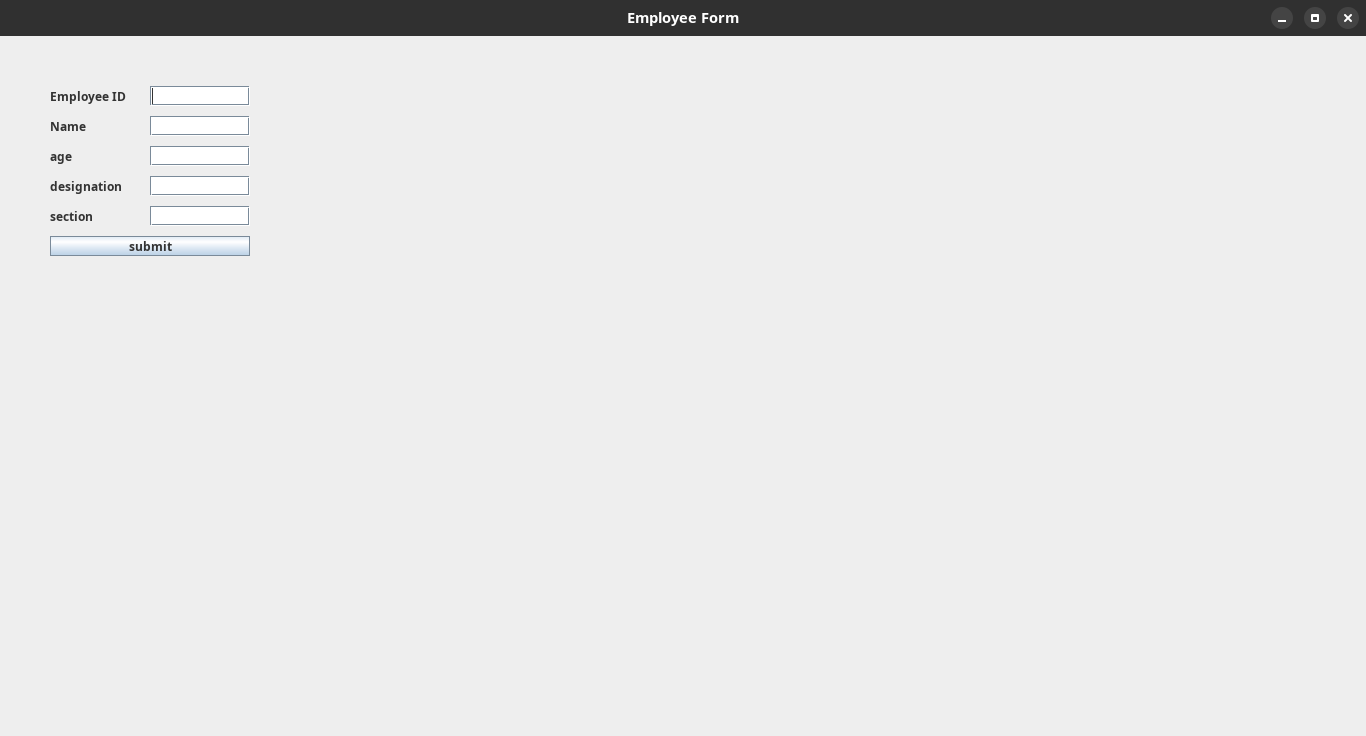
\includegraphics[width=11cm, height=9cm]{./images/01.png}
\end{document}
